\documentclass[two column, twoside, a4paper]{article}

\usepackage[utf8]{inputenc}
\usepackage{paralist}
\usepackage{gensymb}
\usepackage{chemmacros}
\usepackage{booktabs}
\usepackage{dblfloatfix}
\usepackage{url}
\usepackage{subcaption}
\usepackage{float}
\usepackage[backend=biber, maxbibnames=3, style=nature, autocite=inline]{biblatex}
\usepackage[english]{babel}
\usepackage[T1]{fontenc}
\usepackage{fancyhdr}
\usepackage{titlesec}
\usepackage{blindtext}
\usepackage{cuted}
\usepackage{tikz}
\usepackage{enumitem}
\usepackage{booktabs}
\usepackage{hyperref}
\usepackage{newfloat}
\usepackage[referable]{threeparttablex}
\usepackage[most]{tcolorbox}
\usepackage[columnsep = 1cm,
	        lmargin = 0.6in,
	        rmargin = 0.4in,
	        tmargin = 0.5in,
	        bmargin = 0.65in,
	        headsep = \baselineskip]{geometry}

\addbibresource{$BIB}
\renewcommand{\bibfont}{\normalfont\scriptsize}

\renewlist{tablenotes}{enumerate}{1}
\makeatletter
\setlist[tablenotes]{label=\tnote{\alph*},ref=\alph*,itemsep=\z@,topsep=\z@skip,partopsep=\z@skip,parsep=\z@,itemindent=\z@,labelindent=\tabcolsep,labelsep=.2em,leftmargin=*,align=left,before={\footnotesize}}
\makeatother

\hypersetup{
    colorlinks=true,
    linkcolor=cyan,
    citecolor=magenta
  }

\DeclareFloatingEnvironment[name={Supplementary Table},fileext=lst,listname={List of 
Supplementary Tables}]{supptable}

\DeclareFloatingEnvironment[name={Supplementary Figure},fileext=lst,listname={List of 
Supplementary Figures}]{suppfigure}

\raggedbottom

% Custom commands
\newcommand*\circled[1]{\tikz[baseline=(char.base)]{
            \node[shape=circle,draw,inner sep=2pt, color = orange!90!white] (char) {#1};}}

% Section Formatting
\titleformat{\section}
{\sc \bfseries \Large}
{}
{0em}
{}[\vspace{-0.3em}]

\titleformat{\subsection}
{\bfseries}
{}
{0em}
{}

\titleformat{\subsubsection}
{\itshape}
{}
{0em}
{}

% Box formatting
\tcbset{sharp corners, enhanced, colback=white, boxrule = 1pt}

\pagestyle{fancy}
\fancyhf{}
\fancyhead[RE, LO]{University of Warsaw}
\fancyhead[LE, RO]{Faculty of Mathematics, Informatics and Mechanics}
\fancyfoot[RE, LO]{Jakub J. Guzek}
\fancyfoot[LE, RO]{\thepage}
\fancyfoot[CE,CO]{Genomika porównawcza (1000-719GP2)}
\renewcommand{\footrulewidth}{0.05pt}

\begin{document}

\begin{strip}
	{\bfseries \LARGE \fontfamily{phv}\selectfont Phylogenetic pipeline: phylogenetic analysis of chosen species from \textit{Armillaria} genus} \vspace{\baselineskip}

	{\bfseries \large Jakub J. Guzek}

	{University of Warsaw, Faculty of Mathematics, Informatics and Mechanics, Genomika porównawcza (1000-719GP2), \\ Student ID: 456616}\vspace{\baselineskip}

	\hrule\vspace{\baselineskip}

	\textbf{\textsf{Fungi from basidiomycete genus \textit{Armillaria} are responsible for root rot in woody plants in various geographic regions. They are characterized by wide host range, low host specificy and are present on all continents, except Antarctica. They are capable of thriving both in natural forests and on woody crops. Armillaria root rot -- the disease caused by those fungi, can cause serious economic losses when it attacks industrial plantations or orchards. Fungi from this genus, have been the object of interest of many mycologists and plant pathologists for a long time, because of their pathogenicity but also because individuals of \textit{Armillaria} species are among the oldest and largest discovered organisms on earth. This led to multitude of research papers on \textit{Armillaria} physiology, ecology and phylogeny being published over the years. While relatively mature, fungal phylogeny remains a field, that could benefit from more rigorous and extensive analyses of readily available data. As such, most studies of \textit{Armillaria} phylogeny focus on a handful of molecular markers, thus not fully utilizing annotated genomic assemblies. Here I present an analysis of phylogeny, utilizing full proteomic data from 8 species from \textit{Armillaria} genus.}}
	\vspace{\baselineskip}

	\hrule

\end{strip}

\section{Introduction}

Saprotrophic and necrotrophic fungi were shown to be the most efficient decomposers of lingocellulose -- material complex consisting of cellulose, hemicelluloses, lignin and other structural macromolecules, which constitutes the majority of plant biomass\autocite{Harley1971}. Those wood-decaying fungi are essential agents of carbon cycling in forest ecosystems\autocite{Heimann2008}. 

Agaricomycetes are the main group within Basidiomycota, responsible for decay of dead wood\autocite{Krah2018}, with two main modes of dead wood decay that can be distinguished among them: white rot and brown rot. Brown rot fungi have the ability to decompose cellulose and hemicelluloses, but cannot fully degrade lignin. White rot fungi, on the other hand, can decompose cellulose, hemicelluloses and also fully degrade lignin.\autocite{Worrall1997}

  Wood decaying fungi in Agaricomycetes encompass species with very different lifestyles, from mycorrhizal symbiosis, through saprotrophy and necrotrophy to parasitism\autocite{Krah2018} Many fungi are not easily characterized by single lifestyle, and can be mycorrhizal in some circumstances and pathogenic in others. Most of plants on Earth depend on symbiosis with fungi\autocite{Brundrett2018} and some plants are even able to be parasites of fungi\autocite{Leake1994, Bidartondo2002, Merckx2009}. 

  Although it's important to underline the complexity of fungi-plant relationships, which are often impossible to put into simple, discrete categories, this report will use this mentioned classification for simplicity.

  While enzymes encoded in genomes of white rot and brown root fungi allow for decomposition of wood regardless of plant species, it was shown that white rot fungi are more often specializing in decaying wood of angiosperm plants, while brown rot fungi tend to be generalists, able to decay wood from wide range of angiosperm and gymnosperm species.\autocite{Krah2018}

\subsection{Armillaria genus}

Fungi from genus \textit{Armillaria} are plant pathogens that cause root rot. They are present on all continents beside Antarctica\autocite{Coetzee2018} and are generalists able to attack many species of woody plants. Species from this genus are also extraordinarily efficient at colonizing new regions, due to their ability to produce rhizomorphs -- specialized root-like structured composed from vegetative mycelium, which allow the fungus to search for new hosts and for clonal dispersal. Their ability to colonize new areas can be also attributed to the fact, that they are not obligatory pathogens, rather they often act opportunistically and can survive as saprotrophic/necrotrophic white rot fungi in right conditions\autocite{Gregory1985, Morrison2004, Baumgartner2011}. Some species of \textit{Armillaria} were even shown to be symbiotic with plants or be hosts of mycoheterotrophic plants\autocite{Zhan2020, Liu2023}.

\textit{Armillaria} fungi can cause serious economic losses if they attack industrial plantations or orchards. Because of that \textit{Armillaria} have been extensively studied both by academic mycologists and United States Department of Agriculture\autocite{Shaw1991}. Some species of \textit{Armillaria} exhibit bioluminescence, which was additional reason for studying them.\autocite{Ke2020, Oliveira2015}

Individuals of some \textit{Armillaria} species can reach extraordinary sizes. One of such individuals, aptly named "humongous fungus" is one of the largest and oldest known terrestrial organisms on Earth. Lower estimate of its size suggest that it spans 15 hectares and weights at least 10 tons. Its age was estimated to be at lest 1500 years.\autocite{Smith1992}. Newer estimates by Anderson et al. suggest that it might be 2500 years old, and weight at least 40 tons\autocite{Anderson2018}. Individuals of those species might be able to reach such age due to extremely slow mutation rates (magnitudes lower than those of other filamentous fungi\autocite{Anderson2014}.)

\begin{table*}
  \caption{Trophic strategies and geographic range of chosen \textit{Armillaria} species. Adapted from Koch et al. 2017\protect\nocite{Koch2017}}
  \vspace{-1em}
  \label{tab:Armillaria}
  \begin{center}
    \begin{threeparttable}
    \begin{tabular}[c]{lp{0.1\textwidth}p{0.1\textwidth}p{0.28\textwidth}l}
      \toprule
      \textbf{Species} & \textbf{Facultative Necrotroph} &
      \textbf{Rizomorphs in nature} & \textbf{Known range} &
      \textbf{References} \\
      \midrule
      \textit{Armillaria borealis} & Yes & Yes & Europe & \autocite{Gregory1985b, Guillaumin1993, gbif_Armillaria_borealis} \\
      \textit{Armillaria fumosa} & Unknown & Yes\tnotex{tnote:fumosa} & Austalia & \autocite{Morrison2004, Mihail2005, gbif_Armillaria_fumosa} \\
      \textit{Armillaria gallica} & Yes & Yes & Europe, North America, Asia & \autocite{Guillaumin1993, gbif_Armillaria_gallica} \\
      \textit{Armillaria luteobubalina} & Yes & Yes & Australia, Tasmania & \autocite{Coetzee2003, Pareek2001, gbif_Armillaria_luteobubalina} \\
      \textit{Armillaria mellea} & Yes & Yes & Europe, North America, Asia & \autocite{Guillaumin1993, gbif_Armillaria_mellea} \\
      \textit{Armillaria nabsnona} & Yes\tnotex{tnote:nabsnona} & Yes & North America, Hawaii & \autocite{Volk1996, Baumgartner2001, gbif_Armillaria_nabsnona} \\
      \textit{Armillaria ostoyae}\tnotex{tnote:solidipes} & Yes & Yes & Europe, North America, Japan, China & \autocite{Guillaumin1993, Mihail2005, Hasegawa2011, Burdsall2008, gbif_Armillaria_ostoyae} \\
      \textit{Armillaria novae-zelandiae} & Yes & Yes & Argentina, Australia, Chile New Zeland & \autocite{Shaw1977, Shaw1981, Pildain2010, gbif_Armillaria_novae_zelandiae} \\
      \textit{Armillaria solidipes}\tnotex{tnote:solidipes} & Yes & Yes & Europe, North America, Japan, China & \autocite{Guillaumin1993,Mihail2005, Hasegawa2011, Burdsall2008, gbif_Armillaria_solidipes} \\
      \bottomrule
    \end{tabular}
    \begin{tablenotes}
    \item\label{tnote:fumosa}As shown by Morrison et al. (2004) \textit{Armillaria fumosa is able to produce weak rhizomorphs \textit{in vitro}}
    \item\label{tnote:nabsnona}Likely not pathogenic or very weakly pathogenic, as per Baumgartner et al. (2001)
    \item\label{tnote:solidipes}\textit{Armillaria solidipes} is an older name for the \textit{Armillaria ostoyae}. They are the same biological species, and name \textit{Armillaria solidipes} should generally be used. Here, they are distinguished due to them having two different assembly genomes available in GenBank.
    \end{tablenotes}
    \end{threeparttable}
  \end{center}
\end{table*}

\subsection{Motivation}

There is a huge number of published studies on \textit{Armillaria} and closely related genera's physiology, morphology, ecology and phylogeny. Usually motivation for those studies is importance of those fungi as vectors of \textit{Armillaria} root rot disease. Sometimes they are motivated by special interesting quirks of mushrooms from this genus, such as bioluminescence, ability to reach massive sizes and slow mutation rate.

However, a lot of phylogenetic studies of this genus, uses only a handful of molecular markers for reconstruction of phylogenetic trees. In this report I present a resolved phylogeny of 8\footnote{9 proteomes are used, however two of them belong to a single biological species \textit{Armillaria solidipes}} \textit{Armillaria} species, whose annotated genomic assemblies are available in GenBank. Analysis presented here uses full proteomic data for phylogeny inference.

\section{Materials and Methods}

\subsection{Acquisition of proteomes from GenBank}

Annotated genome assemblies were acquired directly from NCBI ftp server using custom Python programs. All chosen proteomes are part of GenBank database (Supplementary Table \ref{tab:proteomes}). Criteria for choice of given assemblies were: (1) availability of protein sequences, (2) date of submission and (3) whether they were tagged as a reference genome or not. Sometimes assemblies tagged as reference either weren't fully annotated or didn't contain protein sequences; in such cases latest annotated assembly was chosen instead.

\subsection{Identification of protein families}

Families of protein sequences for later inference of protein families phylogenetic trees, were calculated using MMseqs clustering method implemented in MMseqs2 program\autocite{Steinegger2017, Steinegger2018, Mirdita2019}. \texttt{cluster} and \texttt{easy-cluster} commands were tested. Other than \texttt{-c} parameter, responsible for setting the minimal threshold for coverage between sequences, default setting were used for \texttt{cluster} command. Three values were tested for \texttt{-c} parameter: 0.75, 0.8 and 0.85; 0.8, which incidentally is the default value was arbitrarily chosen as the best, offering the best balance between the number of identified clusters, number of sequences in clusters and taxa representation within clusters. \texttt{easy-cluster} command, which provides out-of-the-box easy clustering, returned identical results to \texttt{cluster} command.

\subsection{Filtering the obtained clusters}

Clusters were then filtered to get a set of protein families in which every taxon would be represented in each family. Two filtering variants were used: (1) only orthologic sequences (1-1 variant) (2) orthologic and paralogic sequences ("with paralogs" variant).

\subsubsection{1-1 variant}

For 1-1 variant only clusters that contained one sequence per taxon, and included all 9 taxa were used. Out of 53\,290 obtained clusters 3140 fitted those filtering criteria, and those were used for further analyses.

\subsubsection{'with paralogs' variant}

For variant with paralogs, in addition to clusters from 1-1 variant, clusters that included all 9 taxa but had no less than 9 and no more than 29 sequences in total were used. Out of 53\,290 obtained clusters 4527 fitted those filtering criteria, 1387 of which were clusters containing paralogs. 

\subsection{Multialignment and inference of family trees}

For each cluster from filtered subsets, a multiple sequence alignment was inferred using MAFFT\autocite{Katoh2013}, with the following settings: global alignment with 1000 iterations of refinement. Next ML trees with bootstrap supports were inferred for each cluster based on obtained multiple sequence alignments. To do so RAxML Next Generation\autocite{Kozlov2019} was run with empirically calculated stationary frequencies, GAMMA8 model for among-site heterogeneity and LG model\autocite{Le2008} for substitution matrix. One hundred bootstrap replicated were produced for each tree to calculate support of branches. 

LG model was chosen, because its widely used in phylogenetic studies of fungi, and because on average it's better than most other models, while rarely being worse, as was shown in original paper by Le and Gascuel\autocite{Le2008}.

\subsection{Consensus tress}

Consensus trees were calculated from obtained protein family trees using RAxML Next Generation with \texttt{--consense} option. Consensus trees were calculated in two variants: (1) using majority rule with threshold of 50\% and (2) using majority rule with greedy heuristic, which extends majority rule consensus tree by adding the compatible branches with the highest support, until a strictly bifurcating tree is obtained.

\subsection{Supertree}

Supertree was computed using DupTre  program\autocite{Wehe2008} with default parameters. DupTree uses gene tree parsimony. It searches for the species supertree that results in the fewest gene duplication events.

\subsection{Filtering of trees with low support}

Protein family trees containing branches with low support (<0.7) were filtered out. Then consensus and supertrees were computed on this filtered subset of trees, using the method described above.

\subsection{Analysis of protein families with paralogs}

All of the analyses described above were carried out for both 1-1 variant and 'with paralogs' variant, except for construction of consensus trees, which by definition cannot be used as a method to compute genome trees, using trees that contain paralogs.

\subsection{Downstream analysis}

Visualizations of tree comparisons was done using TreeTools and TreeDist libraries for \textsf{R} programming language.

\section{Results}

\subsection{Clustering of sequences}

As expected most of the clusters contained only a small amount of sequences, with majority containing less than five (Supplementary Figure \ref{fig:clustering}b). However majority of the clusters contained around one sequence per unique taxa within cluster (Supplementary Figure \ref{fig:clustering}a) which meant that a lot of clusters contained families of orthologic sequences or families that contained only a small amounts of paralogs.

\subsection{Genome trees}

\begin{figure*}[t]
  \begin{center}
    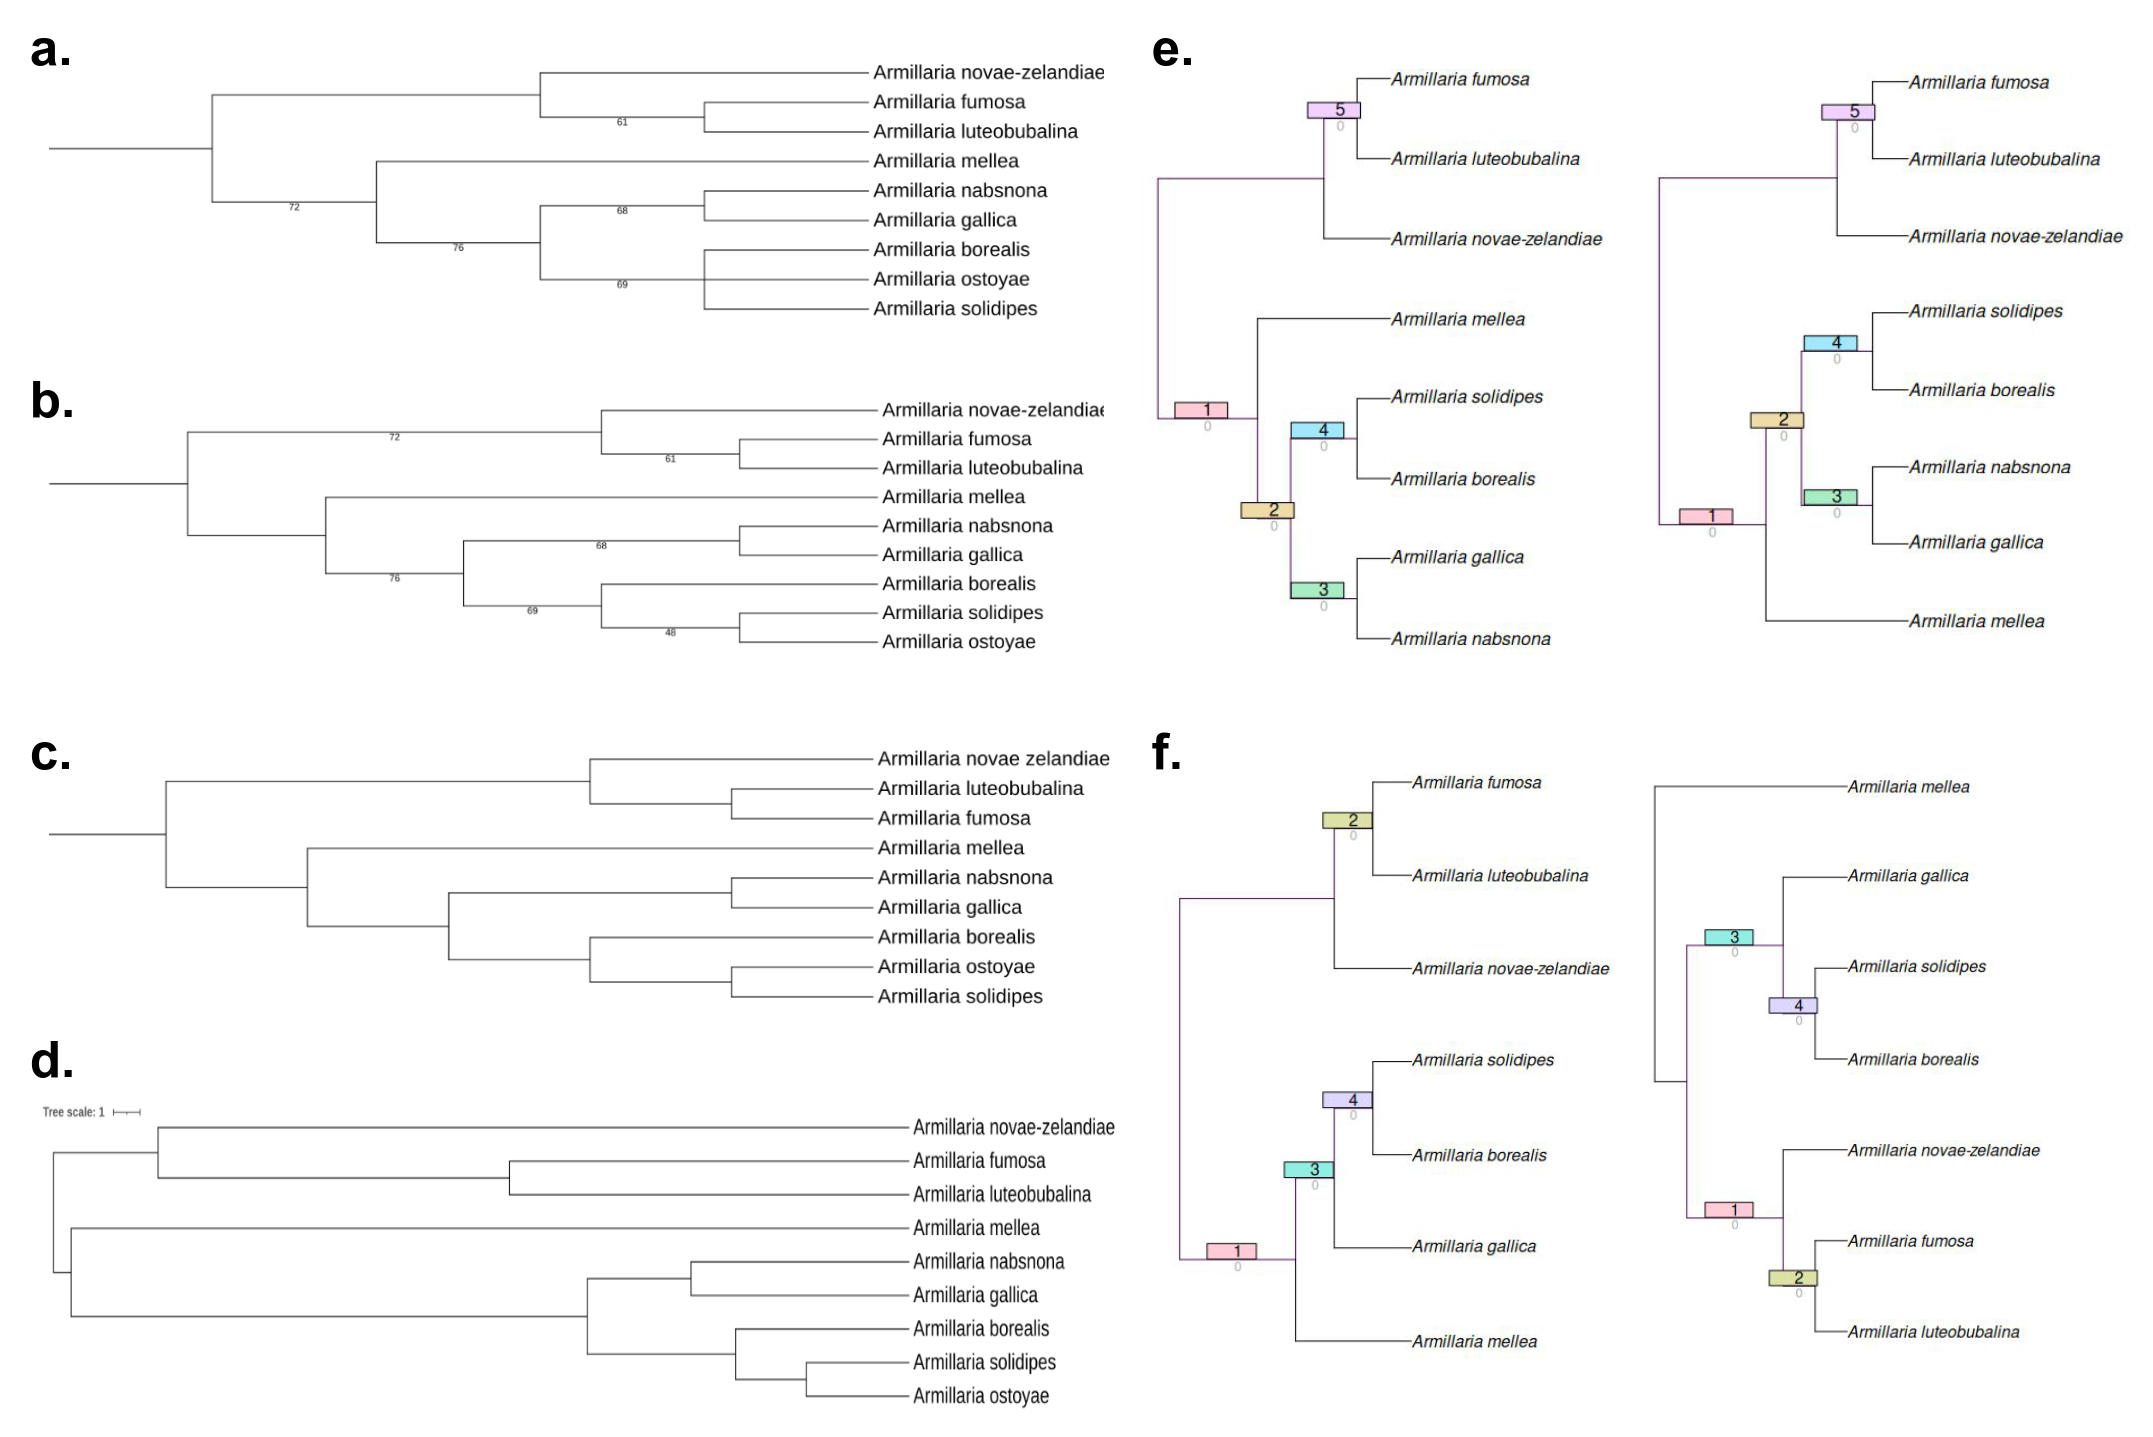
\includegraphics[width=0.98\textwidth]{figures/Figure_2.png}
  \end{center}
  \caption{\sf\textbf{Both greedy majority consensus and supertree are corroborated by timetree and literature data.} \textbf{a.} Rooted majority consensus tree obtained from 1-1 variant ML trees. \textbf{b.} Rooted greedy majority consensus tree obtained from 1-1 variant ML trees. \textbf{c.} Species supertree obtained using DupTree. \textbf{d.} Phylogenetic tree from timetree.org \textbf{e.} Visualization of comparison of MRE tree with \textit{Armillaria} phylogenetic tree adapted from Coetzee et al. 2011\protect\nocite{Coetzee2011}; there is no \textit{Armillaria ostoyae} there, so it was ignored for purposes of comparison. \textbf{f.} Visualization of comparison of MRE tree with \textit{Armillaria} phylogenetic tree adapted from Koch et al. 2017\protect\nocite{Koch2017}; \textit{A. ostoyae} and \textit{A. nabsnona} were skipped for purposes of comparison.}
  \label{fig:trees}
\end{figure*}


Both consensus trees (majority rule with 0.5 threshold -- MR and majority rule with greedy heuristic -- MRE) obtained from variant 1-1, had very similar topology (Fig. \ref{fig:trees}a-b) with only difference being that majority consensus without greedy heuristic produced a tree with multifurcation in \textit{A. borealis} \textit{A. ostoyae} and \textit{A. solidipes} leaf cluster. This is to be expected as the branch that is introduced there in a variant that used greedy heuristic is present in less that 50\% of trees. Species supertree obtained using DupTree program (Fig. \ref{fig:trees}c), had identical topology to the MRE consensus tree.

Phylogenetic tree obtained from timetree\autocite{Kumar2017} (Fig. \ref{fig:trees}d) corroborates the topology of MRE consensus tree and species supertree. All trees were rooted on \textit{A. novae-zelandiae}, \textit{A. fumosa}, \textit{A. luteobubalina} cluster for ease of visual comparison with tree from timetree.org.

To further validate the correctness of resulting genomic trees, MRE consensus tree was compared to trees from literature. MRE consensus tree had identical topology to the abridged \textit{Armillaria} phylogenetic tree obtained by Coetzee et al.\autocite{Coetzee2011} (Fig. \ref{fig:trees}e). \textit{A. ostoyae} was not included in analysis by Coetzee et al., due to it being recognised as synonymous to \textit{A. solidipes}, so it was skipped in this comparison. MRE consensus tree was also compared to abridged phylogenetic tree calculated by Koch et al.\autocite{Koch2017}. Once again MRE consensus tree had identical topology to that of published tree (Fig. \ref{fig:trees}f), except for the fact, that tree obtained by Koch et al. did not contain \textit{A. nabsnona} and similarly to Coetzee et al. did not contain \textit{A. ostoyae}.

All obtained genomic trees, except for the MR consensus tree, had identical topology to the tree from timetree.org (Supplementary Figure \ref{fig:rf}), and to trees adapted from literature, except for missing taxa.

Genomic trees constructed from the subset of family trees, that had only high-supported branches had the same topology as those constructed from unfiltered dataset (Supplementary Figure \ref{fig:filtered_trees}a-c), with a notable exception of majority rule consensus tree, that didn't have a multifurcation, when constructed from filtered dataset (Supplementary Figure \ref{fig:filtered_trees}a). What is also worth noting, is that support values on branches of consensus trees were higher, when those trees were inferred from filtered dataset.

Species supertree obtained from dataset variant with paralogs had the same topology as one obtained from dataset with only orthologic clusters (Supplementary Figure \ref{fig:filtered_trees}d).

\section{Discussion}

Trees obtained in analyses included in this report are rather high quality, and were able to be corroborated by multiple sources. This can be seen as an evidence supporting usage of full proteomic data for phylogenetic inferences. 

Results from herein described analyses are consistent with important papers on \textit{Armillaria} phylogeny, such as the ones by Coetzee and Koch\autocite{Coetzee2011, Coetzee2018, Koch2017}. It's worth noting here that work by Coetzee and Koch included computationally intensive and conceptually difficult Bayesian methods to compute phylogeny, and my analyses were able to reproduce their results using only ML methods. However it needs to be stressed that aims of mentioned studies were broader and thus justified the use of method chosen by authors. 

Usage of full proteomic data is powerful method for resolving phylogeny, but it still has its drawbacks. It is dependent on access to annotated genomic data, which is often not available and it can be computationally intensive if either number of obtained clusters is high, or number of species chosen for the analysis is high. This analysis only includes 8 species and 9 proteomes. To make decisive claims on usefulness of this method for resolving phylogeny of fungi, one would need to first run more extensive study with more species. 

All of the obtained trees were rooted, somewhat arbitrarily on \textit{A. novae-zelandiae}, \textit{A. fumosa}, \textit{A. luteobubalina} cluster, due to the fact that this cluster is consistently separated from the others in various studies\autocite{Coetzee2011, Koch2017, Coetzee2018, Liu2023}, and because that made the visual comparison with tree from timetree.org easier. However this is not fully methodologically sound, and this study would benefit from inclusion of good outgroup like for example \textit{Desarmillaria} or \textit{Guyanogaster}\autocite{Koch2017, Coetzee2018}, which sadly was an afterthought.

One additional aspect, on which studies by Coetzee and Koch focused, was biogeography and radiation of \textit{Armillaria} species. While methods used here do not offer any insight into those topics, resulting tree is consistent with the results from those studies (Supplementary Figure \ref{fig:biogeography}).

\section{Conclusions}

I managed to provide a reproduction of literature results regarding \textit{Armillaria} genus phylogeny, using full proteomic data, simple sequence clustering and ML methods. 

\subsection{Data availability}

All data used for the analyses is non-proprietary and freely available in GenBank under IDs provided within Supplementary Table \ref{tab:proteomes}.

\subsection{Code availability}

All code used for major processing and analysis steps is available in public GitHub repository under following url \url{https://github.com/jakubguzek/Armillaria-phylogeny}. All tools and scripts used are open source and free.

\newpage
\printbibliography

\scriptsize
\pagebreak

\begin{supptable*}
  \caption{IDs and names of annotated assemblies from GenBank chosen for this study.}
  \label{tab:proteomes}
  \begin{center}
    \begin{tabular}[c]{llll}
      \toprule
      \textbf{Species} & \textbf{GenBank ID} & \textbf{Assembly name} & \textbf{Level} \\
      \midrule
      \textit{Armillaria borealis} & \texttt{GCA\_030435635.1} & Armbor1 & Contig \\
      \textit{Armillaria fumosa} & \texttt{GCA\_030407015.1} & Armfum1 & Contig \\
      \textit{Armillaria gallica} & \texttt{GCA\_002307695.1} & Armga1 & Scaffold \\
      \textit{Armillaria luteobubalina} & \texttt{GCA\_030435615.1} & Armlut1 & Contig \\
      \textit{Armillaria mellea} & \texttt{GCA\_030407055.1} & Armmel1 & Contig \\
      \textit{Armillaria nabsnona} & \texttt{GCA\_030407065.1} & Armnab1 & Contig \\
      \textit{Armillaria novae-zelandiae} & \texttt{GCA\_030435655.1} & Armnov1 & Contig \\
      \textit{Armillaria ostoyae} & \texttt{GCA\_900157425.1} & --- & Contig \\
      \textit{Armillaria solidipes} & \texttt{GCA\_002307675.1} & Armost1 & Scaffold \\
      \bottomrule
    \end{tabular}
  \end{center}
\end{supptable*}

\begin{suppfigure*}
  \begin{center}
    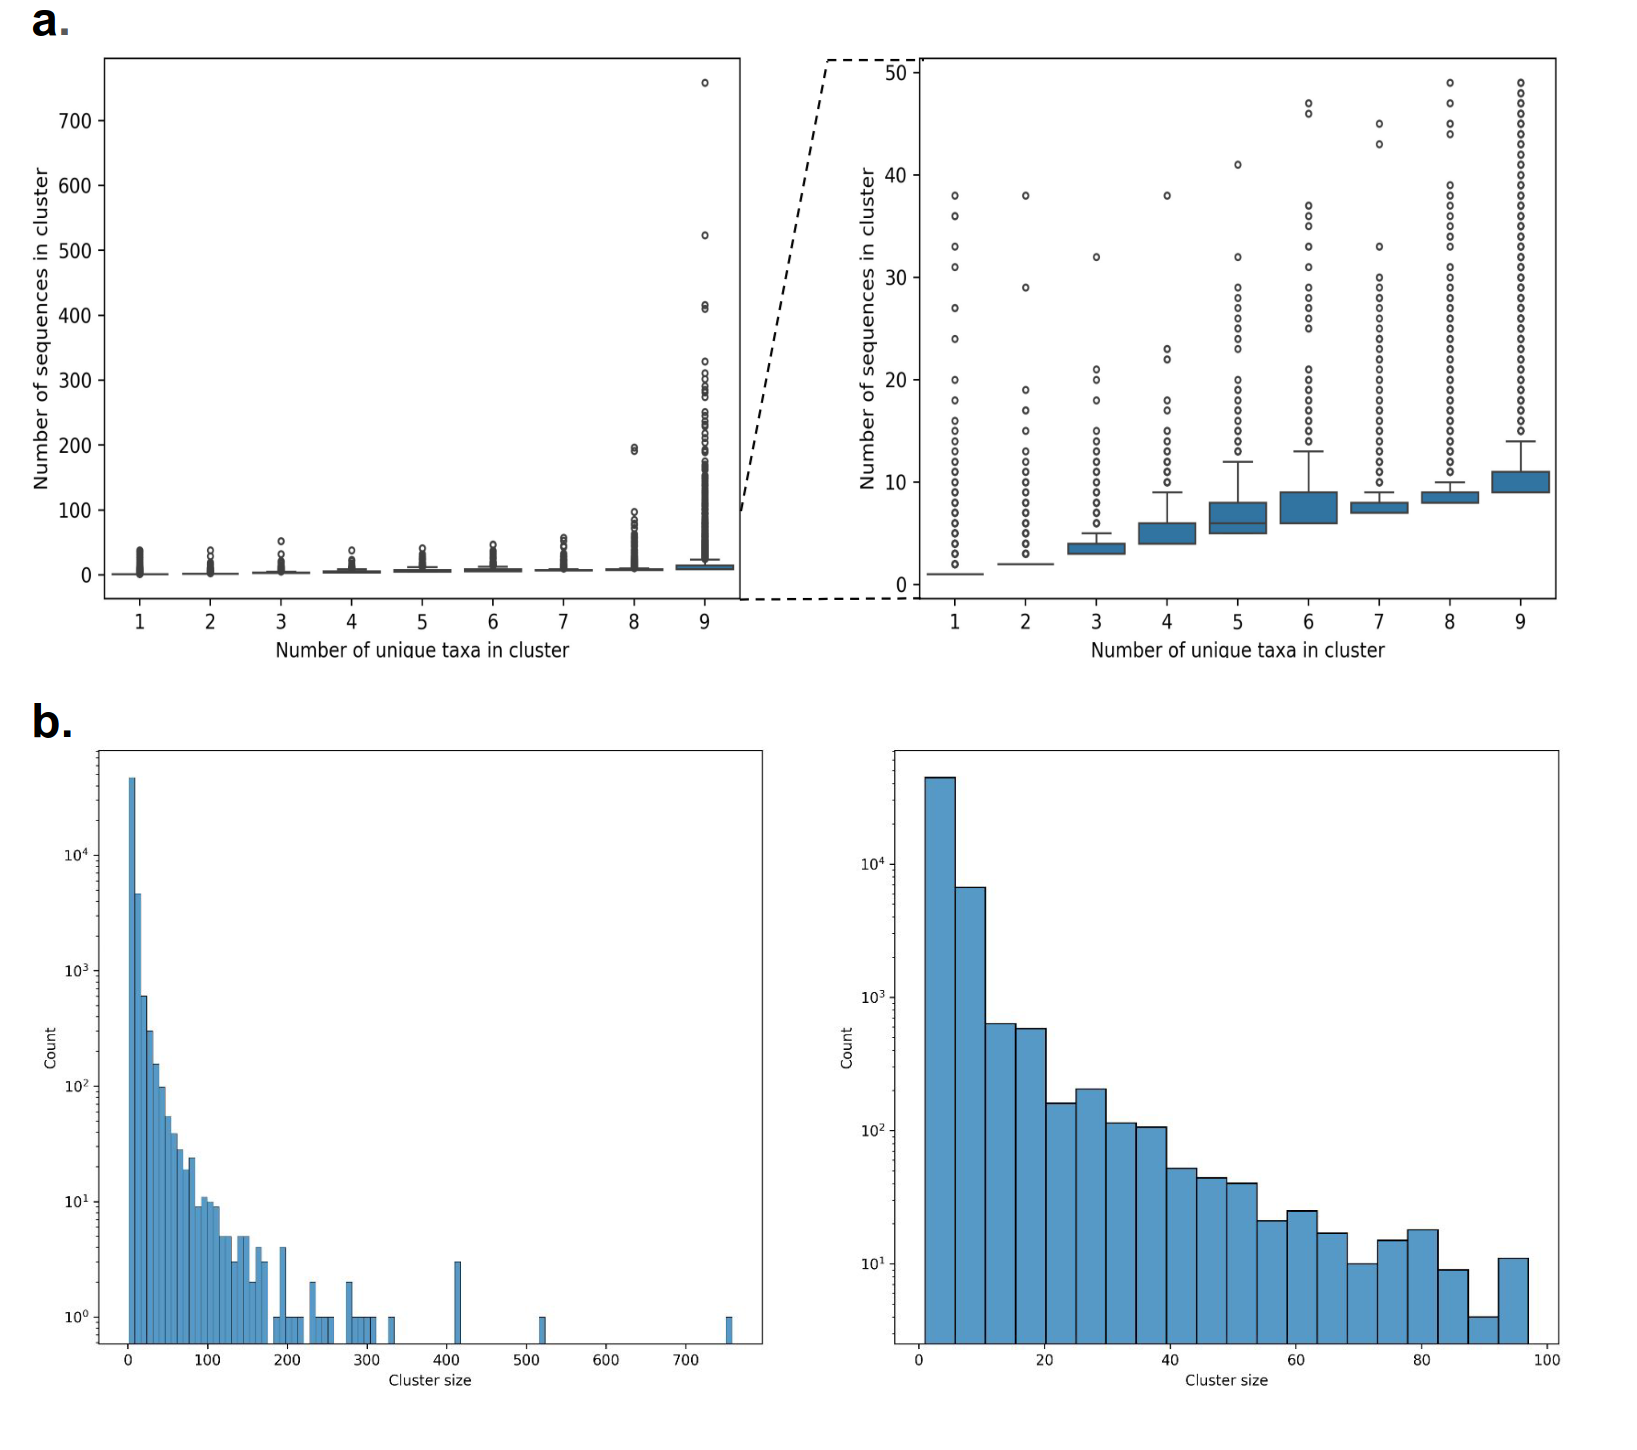
\includegraphics[width=0.95\textwidth]{figures/Figure_1.png}
  \end{center}
  \caption{\sf\textbf{Most clusters contained only one sequence, but majority of those that had 9 unique taxa had around 10 sequences.} \textbf{a.} Box-plot showing the spread of numbers of sequences per cluster in clusters with given number of unique taxa. Most clusters contained one sequence per taxon and only some contained more sequences per taxon, and thus contained no paralogs, or just one or two paralogs \textbf{b.} Histogram of numbers of sequences per cluster. Most clusters contained small number of sequences, but a small amount of clusters contained a lot.} 
  \label{fig:clustering}
\end{suppfigure*}

\begin{suppfigure*}
  \begin{center}
    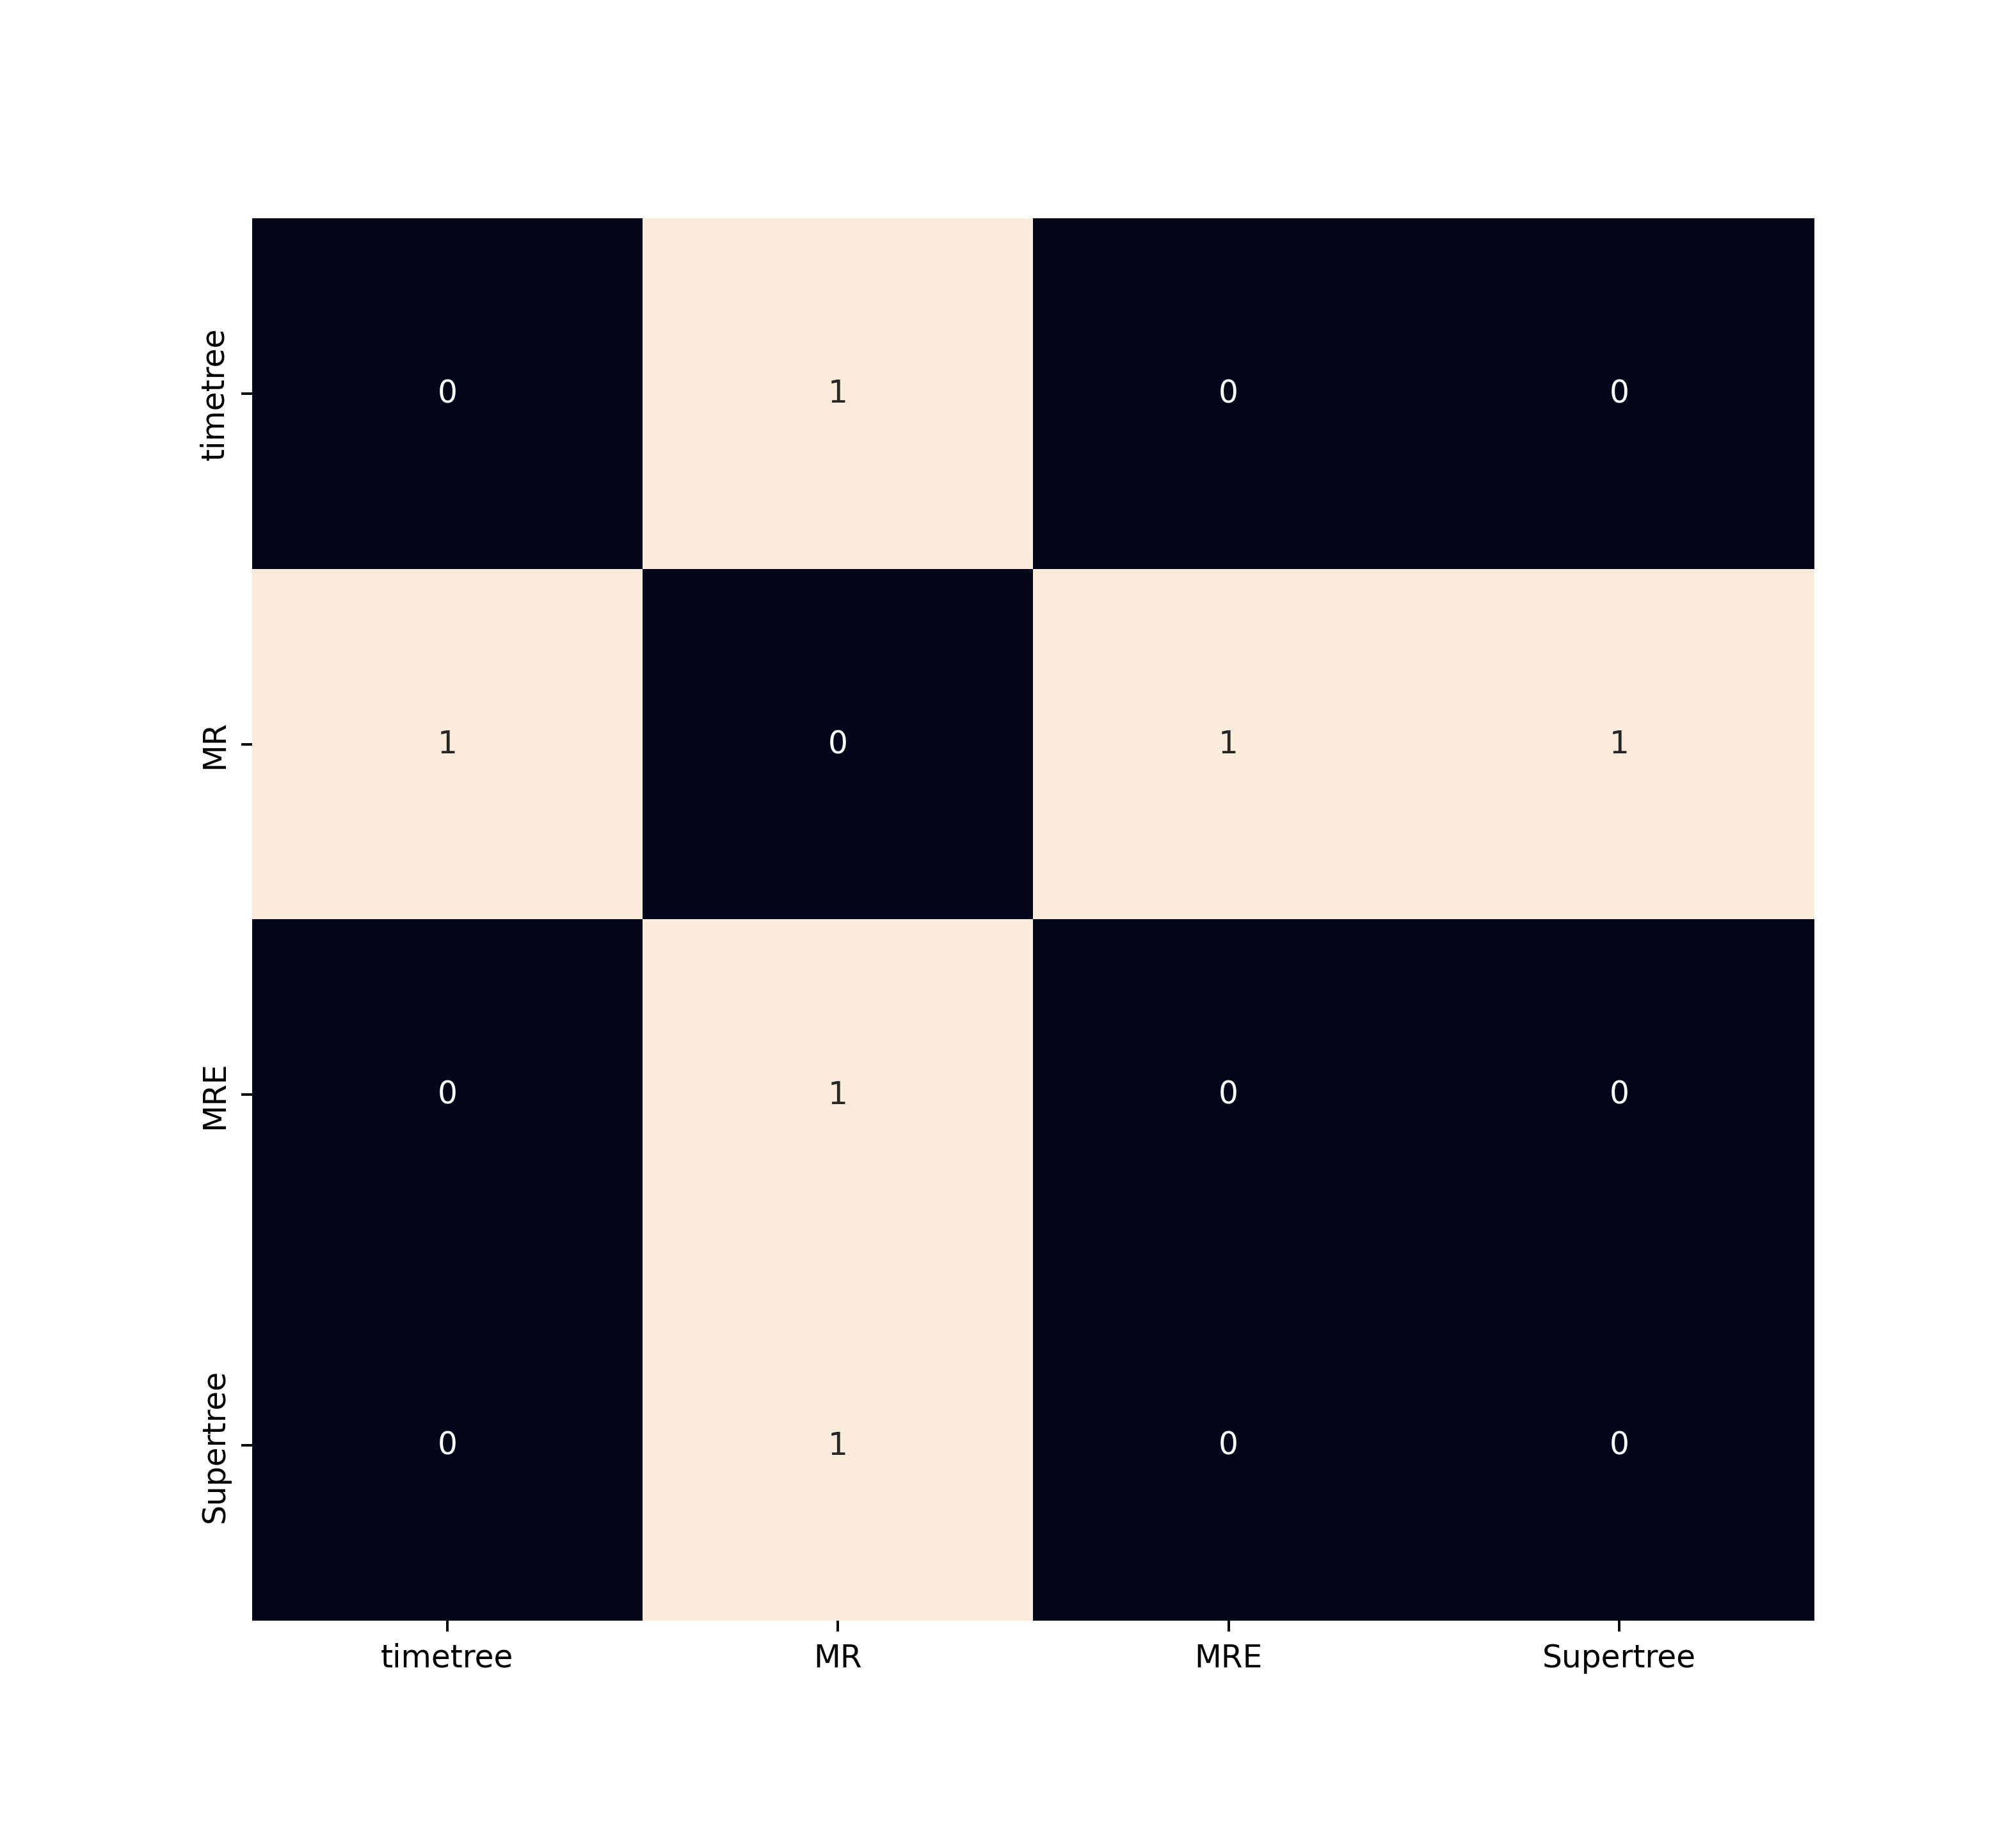
\includegraphics[width=0.95\textwidth]{figures/distances_heatmap.png}
  \end{center}
  \caption{\sf \textbf{Robinson-Foulds distance between all obtained trees, except for MR consensus tree, and timetree was 0}. Heatmap showing distances between trees obtained from variant 1-1 clusters.} 
  \label{fig:rf}
\end{suppfigure*}

\begin{suppfigure*}
  \begin{center}
    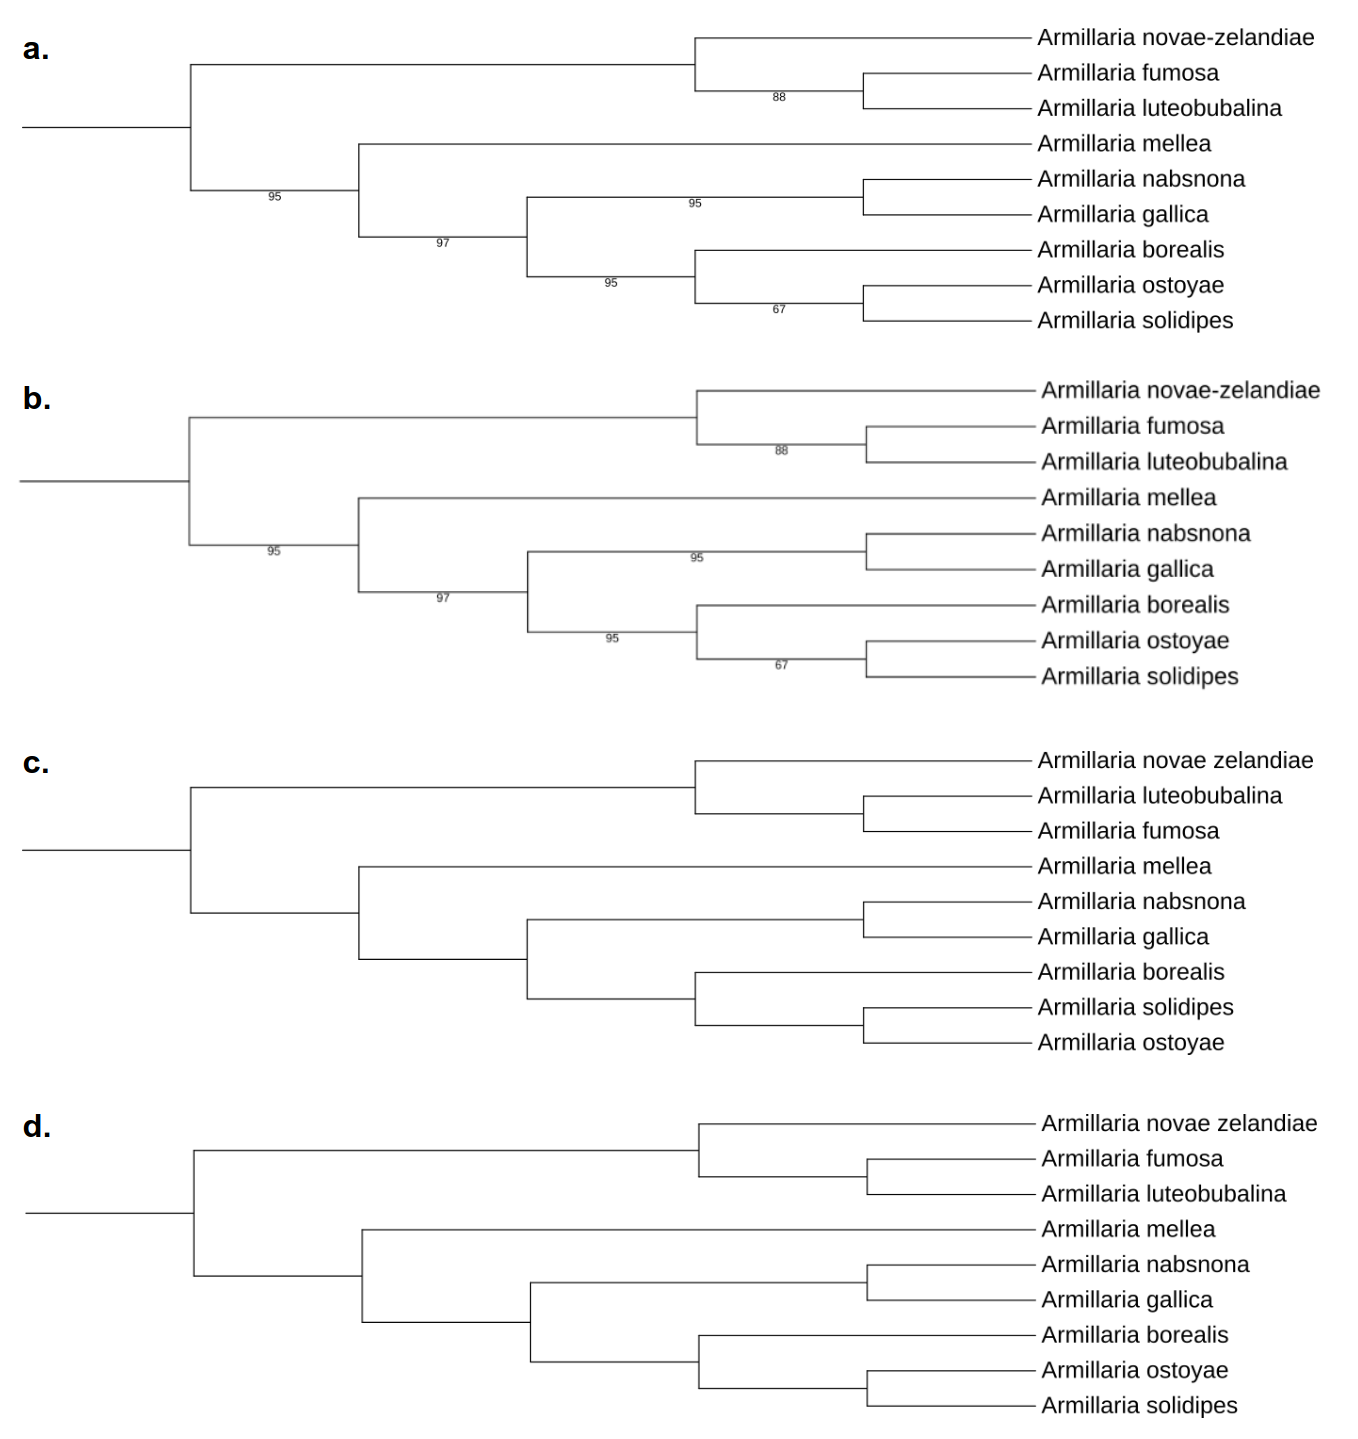
\includegraphics[width=0.95\textwidth]{figures/Figure_3.png}
  \end{center}
  \caption{\sf \textbf{Filtering trees with low-support branches does not impact the topology of resulting genomic trees. Neither does including the clusters with paralogs} \textbf{a.} Rooted majority consensus tree obtained from 1-1 variant after filtering out trees with branches that had low (<0.7) bootstrap support. This is the only tree for which filtering seems to improve the topology as, there is no longer a multifurcation present in \textit{A. ostoyae} \textit{A. solidipes} \textit{A. borealis} cluster. \textbf{b.} Rooted greedy majority consensus tree obtained from 1-1 variant after filtering out tree with branches that had low bootstrap support. \textbf{c.} Rooted species supertree obtained using DupTree from the subset of trees after filtering. \textbf{d.} Species supertree obtained using DupTree from variant with paralogs. As can be observed, the topology of supertree obtained from trees with paralogic sequences is identical to that obtained from tree containing only orthologic sequences.} 
  \label{fig:filtered_trees}
\end{suppfigure*}

\begin{suppfigure*}
  \begin{center}
    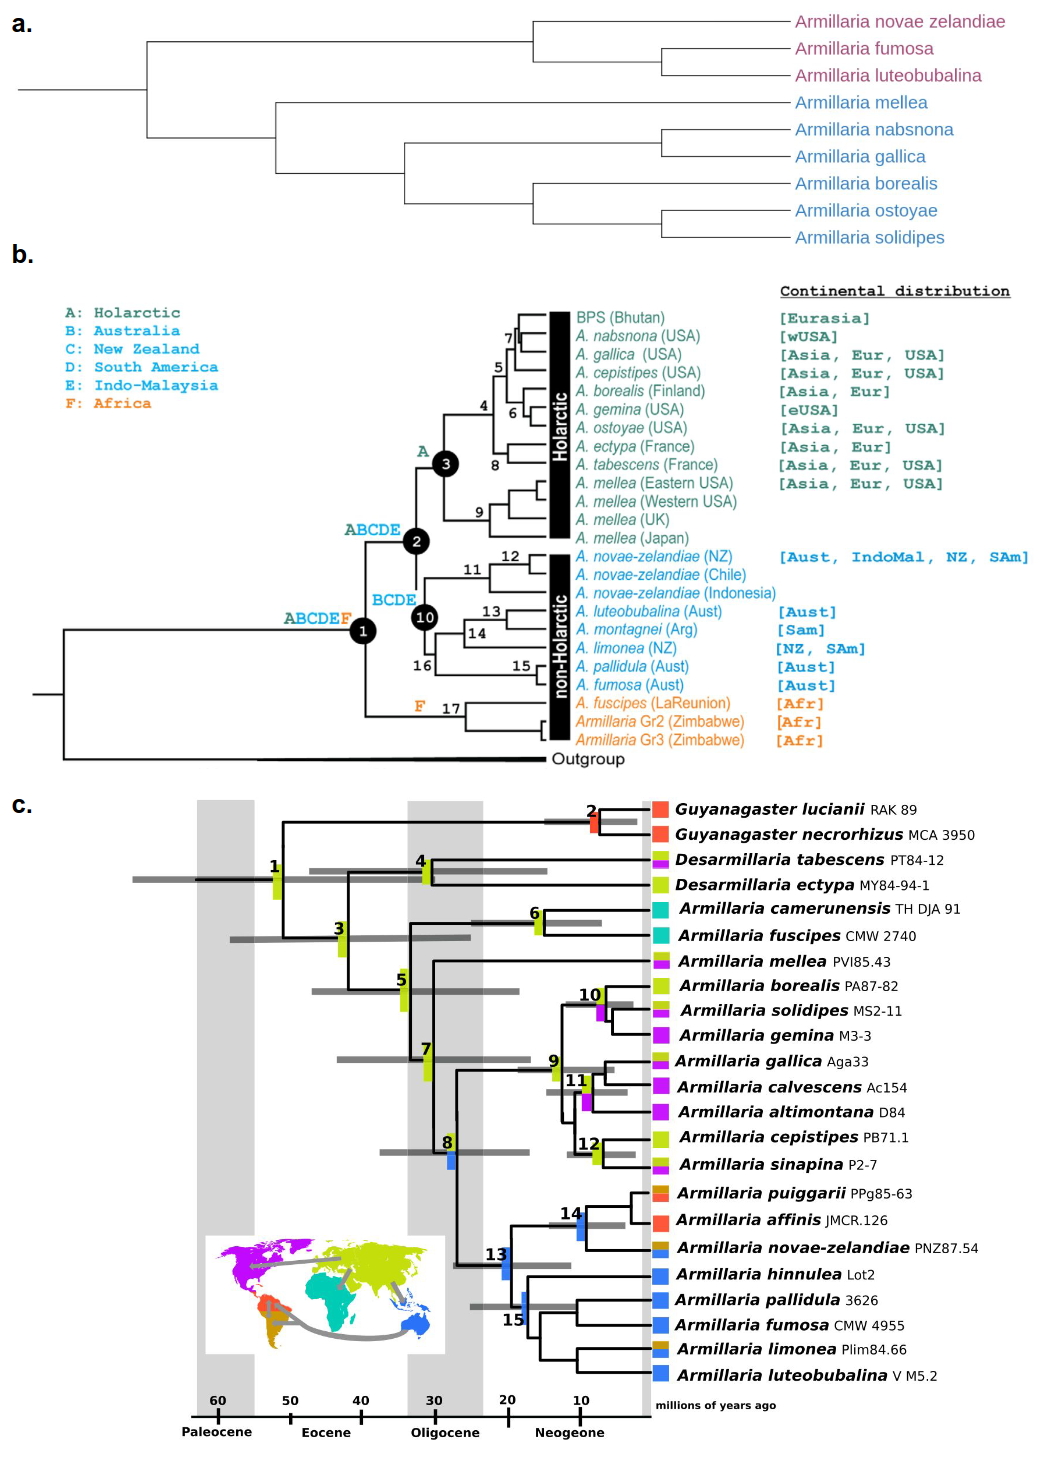
\includegraphics[width=0.95\textwidth]{figures/Figure_4.png}
  \end{center}
  \caption{\sf \textbf{Species supertree is consistent with findings on paleogene radiation and biogeography of \textit{Armillaria} studied by Coetzee et al. and Koch et al.} \textbf{a.} Species supertree with leaves colored by major geographic regions: blue -- Holarctic, purple -- Australia and South America \textbf{b.} Ancestral area recostruction by Coetzee et al. 2011 \textbf{c.} Chronogram with ancestral area reconstruction by Koch et al. 2017} 
  \label{fig:biogeography}
\end{suppfigure*}

\end{document}
